\documentclass{standalone}
\usepackage{tikz,pgfplots,calc,tkz-euclide}
\usetikzlibrary{positioning,calc}
\usetikzlibrary{arrows}
\usepackage{tkz-euclide}
\usetkzobj{all}
\usepackage{amsmath}
\renewcommand{\familydefault}{\sfdefault}

\begin{document}
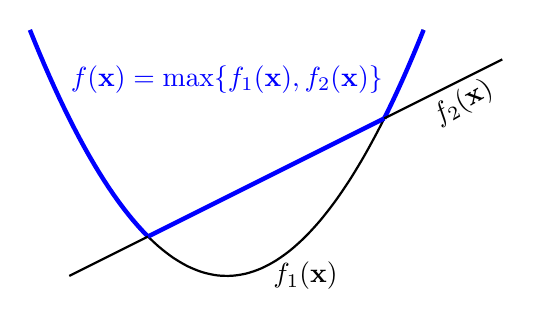
\begin{tikzpicture}[>=stealth, thick]
    \def\a{.3}
    \draw[domain=0:4.5,smooth,variable=\x,black] plot ({\x},{.5*(\x*\x - 4*\x + 4)});      
    \draw[domain=-.5:1,ultra thick,variable=\x,blue] plot ({\x},{.5*(\x*\x - 4*\x + 4)});      
    \draw[domain=4:4.5,ultra thick,variable=\x,blue] plot ({\x},{.5*(\x*\x - 4*\x + 4)});      

    \draw[domain=0:5.5,smooth,variable=\x,black] plot ({\x},{.5*\x});      
    \draw[domain=1:4, draw = blue, ultra thick,variable=\x] plot ({\x},{.5*\x});   

    \node at (3, 0) {$f_1(\mathbf{x})$};   
    \node [rotate = 30] at (5, 2.2) {$f_2(\mathbf{x})$};   
    \node [blue] at (2, 2.5) {$f(\mathbf{x}) = \max \{f_1(\mathbf{x}), f_2(\mathbf{x})\}$};   
    % \foreach \xx in {1}{
    %     \draw[black, thick, domain=(\xx-1):(\xx+2.5),smooth,variable=\x] plot ({\x},{(2*\a*\xx)*(\x - \xx) + \a*\xx*\xx});      
    % }


    % \def\x{1}
    % \def\xp{1.2}
    % \def\xm{-1}
    % \def\y{{\a*\x*\x}}
    % \def\yp{{exp(\a*\xp)}}
    % \def\ym{{exp(\a*\xm)}}

    % \draw [fill = black, draw = black] (\x, \y ) circle (1pt);
    % \node [align = left, scale = .8] at (\x-.5, .5) {$(\mathbf{x}_0, f(\mathbf{x}_0))$};
    % \node [align = left, scale = .8, rotate = 30] at (3, 1.2) {$f(\mathbf{x}_0) + \nabla f(\mathbf{x}_0)^T(\mathbf{x} - \mathbf{x}_0)$};
    % \node [align = left, scale = .8] at (-1.4, 1) {$f(\mathbf{x})$};
    % \node [anchor = west, scale = .8] at (-2, 3) {$f$ is differentiable with convex domain };
    % \node [anchor = west, scale = .8] at (-2, 2.5) {$f$ is convex iff $f(\mathbf{x}) \geq f(\mathbf{x}_0) + \nabla f(\mathbf{x}_0)^T(\mathbf{x} - \mathbf{x}_0), \forall \mathbf{x}, \mathbf{x}_0 \in \text{\bf{dom}}f $};

    % \node [anchor = center, scale = .8] at (0, -1) {convex function};

    % \begin{scope}[xshift = 6cm]
    %     \def\a{.3}
    % \draw[domain=-1.5:2.5,smooth,variable=\x,black] plot ({\x},{.5*(\x*\x - 3*\x +  5*sin(\x r))});      
    % \foreach \xx in {.5}{
    %     \draw[black, thick, domain=(\xx-1):(\xx+1.5),smooth,variable=\x] plot ({\x},
    %     {(\xx - 1.5 + 2.5*cos(\xx r))*(\x - \xx) + .5*(\xx*\xx - 3*\xx +  5*sin(\xx r))});      
    % }

    % \def\x{.5}
    % \def\xp{1.2}
    % \def\xm{-1}
    % \def\y{{.5*(\x*\x - 3*\x +  5*sin(\x r))}}
    % \draw [fill = black, draw = black] (\x, \y ) circle (1pt);
    % \node [anchor = center, scale = .8] at (0, -1) {nonconvex function};

    % \end{scope}
\end{tikzpicture}
\end{document}